\chapter{Kairo -- Das Tor zum Orient}
\noindent\textbf{Ort:} Kairo, Ägypten; Hotel International und Stadtgebiet\\
\textbf{Zeit:} Mai 1920, nach der Reise von Arkham\\
\textbf{Beteiligte:} Francis Collins, Lillie Johnson, Karim el-Mady, Natheniel Moss; Aziz

\begin{meisterinfo}
\textbf{Szenenziel:} Kairo als lebendige Stadt vorstellen, den verlässlichen Übersetzer und Organisator Aziz etablieren, die Ereignisse um Yusuf Hassan rückwirkend verstörend machen und die Reise nach Luxor und zur Ausgrabungsstätte vorbereiten. Aziz ist herzlich, kräftig, lebensfroh und mutig -- und hat eine feste Grenze: Er begleitet die Gruppe bis zum Lager, nicht in die unterirdischen Kammern. Kein einzelner misslungener Wurf darf den Aufbruch verhindern.

\textbf{Kontinuität:} Flynn Carlson und Dr.~Skorbinsk wohnten im Oktober 1919 im Hotel International. Aziz half bei Expedition und Übersetzungen und übernahm Flynns letzten Brief an Helena. Yusuf Hassan ist der verschollene Arbeiter, dem die Ermittler vermeintlich auf dem Atlantik begegneten. Die Zeitphänomene und Zeichen sind noch nicht vollständig erklärt.
\end{meisterinfo}

\section{2.1 -- Ankunft in Kairo}
\begin{figure}[htbp]\centering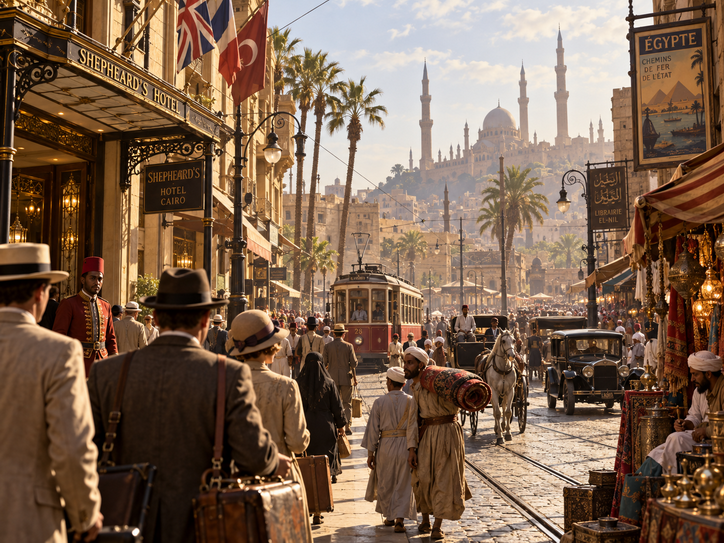
\includegraphics[width=\textwidth]{bilder/kairo-strassenszene.png}\caption{Kairo: Stra\ss{}enbahnen, Wagen, Hotelviertel und das geschäftige Stadtleben. Atmosphärische Illustration, keine historische Fotografie.}\end{figure}
\begin{vorlesetextalle}
Nach der langen Reise erreicht Ihr endlich Kairo. Schon im Bahnhofsgebäude schlägt Euch warme, trockene Luft entgegen. Gepäckträger rufen einander zu, Koffer poltern über Steinplatten, aus vielen Richtungen hört Ihr Gespräche in verschiedenen Sprachen. Unter dem hohen Dach mischen sich die Pfeifsignale der Eisenbahn mit dem Rattern von Handwagen.

Drau\ss{}en erwartet Euch eine Stadt in stetiger Bewegung. Eine Stra\ss{}enbahn rumpelt um die Ecke, ein Automobil hupt hinter einem von Pferden gezogenen Wagen. Händler preisen ihre Waren an, Zeitungsjungen rufen Schlagzeilen, und Menschen in Anzügen, Kleidern, langen Gewändern und unterschiedlichen Kopfbedeckungen drängen sich zwischen Cafés und Geschäften. Über den Dächern zeichnen sich Kuppeln und Minarette ab. Warmer Staub, Gewürze, Tabakrauch und der Duft frisch gebackenen Brotes liegen in der Luft.

Nach Wochen des Reisens erscheint Euch alles gleichzeitig fremd und von beinahe überwältigender Lebendigkeit. Ihr seid in Ägypten angekommen.
\end{vorlesetextalle}
\begin{meisterinfo}
\textbf{Freies Spiel:} Die Gruppe kann Gepäck organisieren, nach dem Hotel fragen, Geld wechseln, den Stra\ss{}enverkehr beobachten oder ein Fahrzeug nehmen. Karim el-Mady kann seine Sprachkenntnisse sinnvoll einsetzen; Ortskenntnis ist damit nicht automatisch gegeben. Keine Pflichtproben. Wer mit Anwohnern spricht, begegnet unterschiedlichen Auffassungen über die politische Lage und ausländische Ausgrabungen, ohne dass daraus ein zusätzlicher Handlungsstrang entstehen muss.
\end{meisterinfo}

\section{2.2 -- Das Hotel International}
\begin{vorlesetextalle}
Euer Wagen hält vor einem stattlichen Hotel mit heller Fassade und breitem Vordach. Gepäckträger eilen herbei. Durch hohe Glastüren gelangt Ihr in eine kühle, gro\ss{}zügige Halle mit Steinboden, dunklen Holzverkleidungen und Messingleuchten. Gro\ss{}e Topfpflanzen flankieren den Empfang. Hoch über Euch bewegen sich Deckenventilatoren träge durch die warme Luft.

Hinter dem Tresen werden Gästebücher aufgeschlagen, Zimmerkarten gereicht und Koffer auf kleine Wagen geladen. Aus einem Salon dringen gedämpftes Stimmengewirr und das Klirren von Teegläsern. Nach den vielen Reisetagen wirkt dieser Ort beinahe unwirklich komfortabel.
\end{vorlesetextalle}
\begin{meisterinfo}
Die Miskatonic University hat Zimmer reserviert. Das Hotel ist ein fiktiver beziehungsweise abenteuerinterner Schauplatz; die Illustration der Stra\ss{}enszene zeigt ein anderes reales Hotel und dient nur der Atmosphäre. Eine Nachfrage beim Empfang bestätigt die Aufenthalte von Flynn Carlson und Dr.~Skorbinsk im Oktober 1919. \textbf{Bibliotheksnutzung (im Register) oder Überreden/Charme (beim Personal):} Ein Angestellter erinnert sich an Skorbinsks häufige Besuche und seine ungehaltenen Nachfragen nach Post; Flynn wirkte freundlicher, aber zuletzt angespannt. Diese Informationen sind fakultativ und dürfen auch ohne Probe durch höfliches Nachfragen zugänglich sein.
\end{meisterinfo}

\section{2.3 -- Aziz stellt sich vor}
\begin{figure}[htbp]\centering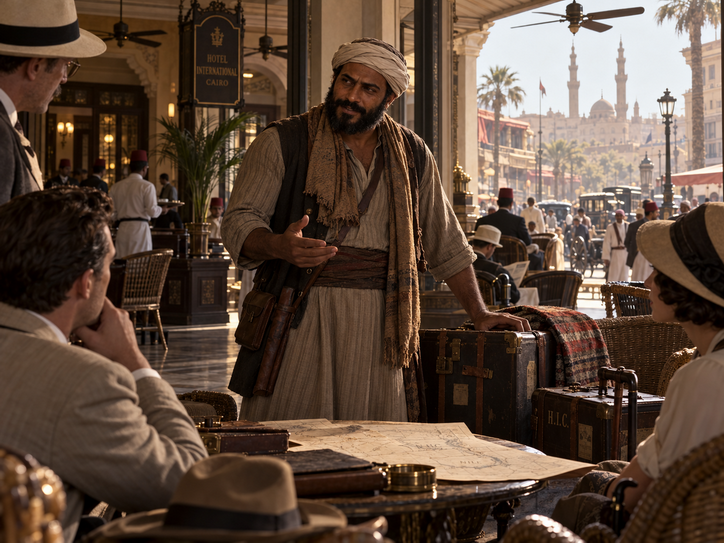
\includegraphics[width=\textwidth]{bilder/aziz-hotel-international.png}\caption{Aziz begrü\ss{}t die Ermittler im Hotel International -- ein kräftiger, humorvoller Mann mit Lebenserfahrung.}\end{figure}
\begin{vorlesetextalle}
Im Salon habt Ihr gerade Platz genommen, als ein kräftiger, breitschultriger Mann mit dichtem dunklem Bart und sonnengebräuntem Gesicht auf Euch zukommt. Seine Kleidung ist zweckmä\ss{}ig, seine Umhängetasche sichtbar viel benutzt. Ausgeprägte Lachfalten umrahmen die Augen, die Euch wach und neugierig mustern.

Der Mann breitet die Arme aus, als begrü\ss{}e er alte Freunde. 

\glqq{}Meine Freunde! Ihr müsst die Herrschaften von der Miskatonic University sein!\grqq{}

Er lacht, reicht Euch nacheinander die Hand und stellt sich vor: \glqq{}Aziz. Einfach Aziz! Ich habe mit Euren Professoren gearbeitet. Mit Carlson und mit diesem anderen Herrn ... Skorbinsk! Bei Allah, dieser Mann konnte einen zur Verzweiflung bringen!\grqq{}

Er winkt einem Kellner. \glqq{}Tee für uns! Und etwas zu essen. Meine neuen Freunde sehen aus, als hätten sie eine lange Reise hinter sich.\grqq{} Dann setzt er sich mit einem zufriedenen Seufzen. \glqq{}Nun erzählt: Was führt Euch in unser schönes Kairo? Doch wohl nicht nur die Aussicht auf guten Tee?\grqq{}
\end{vorlesetextalle}
\begin{meisterinfo}
\textbf{Aziz (etwa 40):} Kräftig, bärtig, lebensfroh, handfest, laut lachend, ortskundig, erfahren in Übersetzung und Reiseorganisation. Er nimmt die Gruppe ernst und behandelt sie zunächst als Gäste. Er ist kein eingeschüchterter Überlebender und kein heimlicher Gegner. Er scherzt über Dr.~Skorbinsks Verschlossenheit, respektiert Flynn und hält nichts davon, Warnzeichen zu ignorieren. Er erklärt von sich aus, dass er die Expedition bis zum Lager begleitet hatte und zuletzt mit Flynns Brief abreiste.

\textbf{Psychologie (regulär):} Beim Thema Katakomben wird Aziz ernst, nicht ängstlich: Er wägt seine Worte ab, weil er die Gefahr nicht leichtfertig kleinreden möchte. Bei Fehlschlag ist die Veränderung seines Tons dennoch bemerkbar.
\end{meisterinfo}
\subsection{Das Gespräch über die Ausgrabung}
\noindent\textbf{Aziz auf Fragen nach dem Ort:}
\begin{quote}\glqq{}Hört zu, meine Freunde. Ich habe Sandstürme erlebt, die ganze Karawanen verschlucken können, und Männer getroffen, die gefährlicher sind als Schlangen. Aber dort unter den Felsen stimmt etwas nicht. Ich wei\ss{} nicht, was es ist. Und ich will es auch gar nicht wissen. Ein vernünftiger Mann hört auf seinen Verstand.\grqq{}\end{quote}
\noindent\textbf{Aziz über die Wissenschaftler:}
\begin{quote}\glqq{}Carlson wollte Antworten. Skorbinsk glaubte schon, sie zu besitzen. Das ist ein gro\ss{}er Unterschied.\grqq{}\end{quote}
\begin{meisterinfo}
Aziz berichtet ohne Probe: Arbeiter verlie\ss{}en den Ort, in der Anlage ertönten unerklärliche Geräusche, Skorbinsk wurde zunehmend verschlossen, Flynn blieb zurück. Er kennt die Anlage nicht vollständig und behauptet nicht, das Rätsel lösen zu können. Auf konkrete Fragen nach dem sehenden Stein berichtet er nur von Skorbinsks Fixierung auf einen Gegenstand; dessen Funktion kennt er nicht.
\end{meisterinfo}

\subsection{Yusuf Hassan -- die Erinnerung an das Schiff}
\noindent\textbf{Falls die Ermittler Yusuf erwähnen:}
\begin{quote}\glqq{}Yusuf Hassan? Ja, ich kannte Yusuf. Ein guter Junge, flei\ss{}ig und immer zu Scherzen aufgelegt. Er ging in die unteren Kammern und kam nicht wieder zurück. Wir haben gesucht. Niemand hat ihn seitdem gesehen.\grqq{}\end{quote}
\noindent\textbf{Nach dem Bericht über die Begegnung im Nebel:}
\begin{quote}\glqq{}Nein, das kann nicht sein. Yusuf war nicht auf Eurem Schiff.\grqq{}\end{quote}
\begin{meisterinfo}
Aziz wird still und mustert die Gruppe, ohne in Panik zu geraten. Dann: \glqq{}Vielleicht solltet Ihr mir genauer erzählen, was Ihr gesehen habt.\grqq{} Ein gelungenes \textbf{Überreden, Charme oder Psychologie} kann zu einer genaueren Beschreibung Yusufs und der Umstände seines Verschwindens führen. Falls die Gruppe nicht von Yusuf berichtet, bleibt dieser Gesprächsteil aus; der Zusammenhang kann später am Lager wieder aufgegriffen werden. Ein Foto der Expeditionsmannschaft wäre ein mögliches späteres Handout, ist derzeit jedoch nicht Bestandteil der vorhandenen Materialien.
\end{meisterinfo}

\section{2.4 -- Aziz' Bedingungen}
\begin{vorlesetextalle}
Aziz stellt sein Teeglas ab und legt die breiten Hände auf den Tisch.

\glqq{}Also gut, meine Freunde. Ich bringe Euch nach Luxor. Ich besorge die Wagen, die Leute und alles, was Ihr braucht. Wenn Ihr darauf besteht, führe ich Euch bis zum Lager.\grqq{}

Er hebt einen Finger. \glqq{}Aber dort ist Schluss. Ich werde keinen einzigen Schritt in diese verfluchten Gänge setzen. Versteht mich nicht falsch: Ich bin kein Feigling. Aber es gibt einen Unterschied zwischen Mut und Dummheit.\grqq{}

Ein warmes, entschlossenes Lächeln kehrt auf sein Gesicht zurück.

\glqq{}Ihr wollt Carlson finden? Dann helfe ich Euch. Doch mit den Dingen, die dort unten geschehen, will ich nichts zu tun haben.\grqq{}
\end{vorlesetextalle}
\begin{meisterinfo}
\textbf{Spielmechanik:} Aziz' Begleitung bis zum Lager steht fest; eine Probe auf Überreden oder Charme ist dafür nicht notwendig. Gute Argumente und gelungene soziale Proben können ihm zusätzliche Erklärungen, Kontakte, eine Reserveausrüstung oder einige weitere Tage Logistik am Lager entlocken. \textbf{Unverrückbar:} Er betritt weder die Grabkammer noch die Katakomben. Das ist eine begründete Entscheidung eines erfahrenen Mannes, keine Feigheit. \textbf{Falls die Gruppe ihn bedrängt:} Er bleibt freundlich, wird aber bestimmt: \glqq{}Meine Antwort bleibt nein.\grqq{}
\end{meisterinfo}

\section{2.5 -- Das Zeichen an der Zimmertür}
\begin{vorlesetextalle}
Spät am Abend ist das Hotel ruhig geworden. Von der Stra\ss{}e dringt nur noch ein gedämpftes Rauschen herauf. Dann hört Ihr drei langsame Schläge gegen Holz.

Als Ihr die Zimmertür öffnet, ist der Gang leer. Die Wandlampen werfen gelbliche Lichtinseln auf den Boden. Unmittelbar vor der Schwelle liegt eine feine Spur Sand. Sie führt ein paar Schritte weit und endet ohne erkennbare Fortsetzung.

Auf der Innenseite der Tür seht Ihr etwas, das Euch zuvor nicht aufgefallen ist: ein in das Holz eingeritztes Zeichen, ein Oval mit einem Punkt darin und einem gebogenen Fortsatz darunter. Ihr kennt dieses Symbol bereits.
\end{vorlesetextalle}
\begin{meisterinfo}
\textbf{Verborgenes Erkennen oder passende Handwerksfertigkeit (regulär):} Die Kerben sind dunkel und wirken erstaunlich alt, nicht frisch eingeschnitten. Der Sand ist feinkörnig und trocken. Weitere Recherchen bei der Nachtschicht führen zu keinem beobachteten Besucher. Am Morgen ist das Zeichen verschwunden; die Tür ist glatt, und auch die Sandspur fehlt. \textbf{Stabilität:} 0/1W3 STA, sobald die Ermittler die Unmöglichkeit des Vorfalls begreifen. \textbf{Inszenierung:} Kein weiteres Gespenst, keine Verfolgung. Die kurze Störung setzt das wiederkehrende Motiv von gestörtem Raum und Zeit fort und sollte nicht vorzeitig erklärt werden.
\end{meisterinfo}

\section{2.6 -- Die Vorbereitungen für die Wüste}
\begin{figure}[htbp]\centering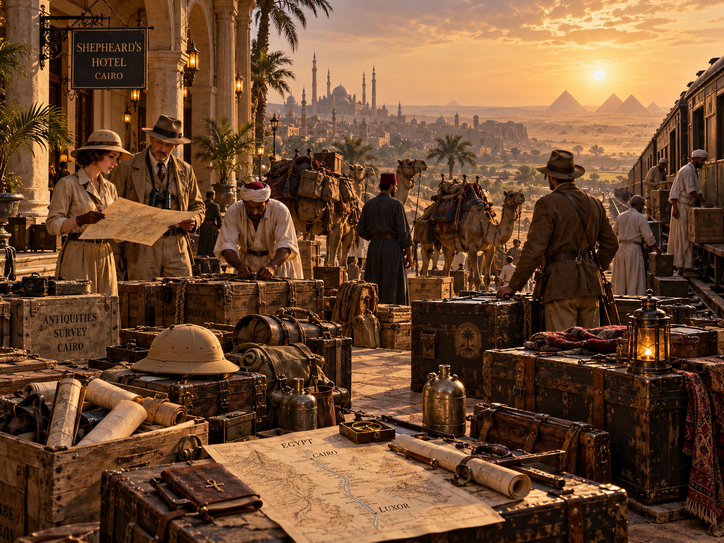
\includegraphics[width=\textwidth]{bilder/kairo-expeditionsvorbereitung.png}\caption{Vorbereitungen für den Aufbruch nach Luxor: Proviant, Werkzeug, Karten und Transportmittel. Atmosphärische Illustration.}\end{figure}
\begin{vorlesetextalle}
Am nächsten Morgen herrscht geschäftiges Treiben. Aziz steht zwischen Koffern, Holzkisten und aufgerollten Decken, prüft Lieferlisten und gibt mit lauter Stimme Anweisungen. Zwischendurch scherzt er mit den Trägern, klopft einem Fuhrmann auf die Schulter und überprüft selbst den Verschluss einer Wasserkiste.

Als er Euch bemerkt, lacht er. \glqq{}Gut! Ihr seid also wach. Ich kümmere mich um die Reise. Ihr kümmert Euch darum, nicht allzu viel unnötigen Unsinn einzupacken. In der Wüste werdet Ihr jedes überflüssige Pfund verfluchen!\grqq{}

Er zeigt auf Karten, Proviant und Ausrüstung, die in sorgfältigen Reihen bereitliegen. \glqq{}Jetzt esst erst einmal ordentlich. Wer wei\ss{}, wann Ihr wieder eine anständige Mahlzeit bekommt!\grqq{}
\end{vorlesetextalle}
\begin{meisterinfo}
\textbf{Grundausstattung:} Aziz organisiert Wasserbehälter und Reservewasser, haltbaren Proviant, Zelte, Decken, Petroleum- oder Öllampen samt Brennstoff, Seile, Werkzeuge und geeignete Transportmöglichkeiten. Er empfiehlt zudem Sonnenschutz, festes Schuhwerk und eine kleine medizinische Ausrüstung. Die Gruppe kann selbst zusätzliche Dinge beschaffen (etwa Fotografieausrüstung, Messgeräte, Skizzenmaterial, weitere Lampen). \textbf{Eigene Entscheidungen:} Sinnvolle Sonderwünsche dürfen Kosten oder Zeit verlangen, sollen aber nicht die Haupthandlung blockieren.

\textbf{Reiseplan:} Zunächst geht es nach Luxor; von dort führt Aziz die Ermittler weiter zum Lager. Die Distanz und der genaue Zeitbedarf dieser letzten Etappe werden mit der nächsten Szene festgelegt. \textbf{Übergang:} Szene 3 -- Das verlassene Expeditionslager.
\end{meisterinfo}
